\documentclass[12pt, a4paper, titlepage]{article}
\usepackage[utf8]{inputenc}

\usepackage{amsmath}
\DeclareMathOperator*{\argmax}{arg\,max}

\usepackage{float}
\usepackage{datetime}
\usepackage{enumitem}
\usepackage{varwidth}
\usepackage{graphicx}
\usepackage{multirow}

\usepackage{geometry}
\geometry{top=1in, left = 1in, right = 1in}

\setlength{\parindent}{0cm}


\title{Agents and Multi-Agent Systems Notes}
\date{\today}
\author{Vishnu}


\begin{document}

\maketitle

\tableofcontents

\section{Introduction}

Computer vision is the extracting of useful information from images. 

\subsection{Related Disciplines:}
\begin{description}
    \item[Image Processing] Manipulating images
    \item[Computer Graphics] Synthesising images
    \item[Pattern Recognition] Recognising and classifying info from datasets/images
    \item[Photogrammetry] Obtaining measurements (e.g height) from images
    \item[Biological Vision] Understanding visual perception in humans/animals \\ \quad \quad  (combines neuroscience, psychology and biology)
\end{description}

\subsection{Difficulties}
Vision exists for specific domains (e.g. the Hawkeye tennis system), but making a general system that works in any environment is an ongoing problem.  

\begin{enumerate}
    \item To a machine, images are an X by Y grid of numbers - even humans would have difficulty
    \item Understanding a 2d image of a 3d object is an ill-posed problem
    \item A single 3d object can have an exponential number of different images (viewpoints, scale, colour,...)
\end{enumerate}

\subsubsection{Ill-Posed Problem}
An \emph{ill-posed problem} is one with more than one potential answer/no answer/no direct relationship between the answer and initial conditions. \\

Converting a 3d image to 2d is well-posed (e.g. looking at a cube head on makes it a square). Converting a 2d to 3d is an inverse problem, so is ill-posed - a single 2d image could have come from multiple different sources (e.g. a square could be one face of a cube or the base of a square pyramid).\\

By using prior knowledge/context, we can interpret the most likely object for an image.

\subsubsection{Exponential images}
For any object in an image, it can appear at any position/scale/orientation/colour/deformation/etc. so there are an exponential number of possible images for an object.\\
Illumination can greatly vary the object's appearance, even if the object itself hasn't changed. There can also be multiple types of the same object (e.g. smartphones), or different classes of objects can look very similar (e.g. calculators and remotes).\\
In more complex images, multiple objects can occlude/cover parts of each other - this not only deforms the object, but provides lots of background noise. 

\subsection{Prior Assumptions}
Using invariant prior knowledge, we can apply these to images to make better sense of them. The brain has a number of prior assumptions (e.g. the effect of shadows and illumination) that it uses to process images. 

Some other priors the brains uses are: perspective, context, prior knowledge and temporal context. We can classify these as:
\begin{enumerate}
    \item Familiarity - general knowledge. e.g if something is further away, we compensate the fact that it looks smaller
    \item Priming - the immediately preceding sensory input. e.g if we just saw a vase on the table, we expect it to be there
    \item Context - information about the surrounding scene. e.g. if we see a keyboard and mouse, we expect to see a monitor nearby
\end{enumerate}
There are visual illusions that show us some of the assumptions that human vision makes - these are usually correct, and have been applied to many specialised vision systems. 

\section{Practical Reasoning}

\subsection{Definition}
\textbf{Practical Reasoning} is reasoning on what actions to do. 

In humans, there are two steps:
\begin{enumerate}
    \item Deliberation - Deciding the desired goal
    \item Means-End Reasoning - Deciding how to achieve the goal
\end{enumerate}

\subsection{Intentions}
Intentions are the result of deliberation: a state of affairs that the agent aims to achieve. Once obtained, agents will devote resources to trying to achieve it. 

For an intention I chosen by an agent A:
\begin{itemize}
    \item A will try to achieve I, trying alternative plans if it fails
    \item A won't aim for any intention that conflicts with I (This helps constrain the search space)
    \item A \emph{believes} that I is possible under certain circumstances 
    \item Agents won't choose intentions that are impossible or that will happen inevitably (without the agent acting)
    \item Agents don't always intend the side effects of their intentions (i.e if a is intended and a$\rightarrow$b, the agent doesn't necessarily intend b) 
\end{itemize}

Intentions can be thought of as a want/goal with actions being put towards it, rather than just a desire. 

\subsection{Planning}
Means-End reasoning gives a plan of action for the agent to achieve its intention, taking into account the environment/state and possible actions.

The largest problem is that deliberation/reasoning aren't instantaneous: the optimal intention may have changed (change in environment/goals) before the deliberation has even finished (Calculative Rationality). 

\subsubsection{Deliberation}
\begin{enumerate}
    \item Generate options/desires using state, environment and current goals (to avoid\\ conflict of intentions)
    \item Filter these options to generate the new intention set
\end{enumerate}

\subsubsection{Commitment}
Once an intention has been selected, the agent \emph{commits} to achieving it.
\begin{description}
    \item [Blind/Fanatical] Commits until the intention is achieved
    \item [Single-Minded] Till achieved or no longer possible to achieve
    \item[Open-Minded] Commits while it believes the intention to be possible
\end{description}

Agents can commit to ends(goals) or means(the actions taken). If there's a change, the agent needs to check if its plan is valid and potentially re-plan.

\subsubsection{Re-consideration Strategies}
\begin{itemize}
    \item Agents can re-check actions/intentions after each action it performs to check they're still possible (open-minded), but this is very costly.
    \item Checking every iteration might cause the agent to only deliberate and never act 
    \item Checking too infrequently might lead the agent to try to achieve something that's no longer possible
\end{itemize} 

Many systems have a higher-level check to determine if the intention/plan should be reconsidered - this check is less costly than reconsidering.

An environment that changes frequently favours constant re-checking, while static environments favour agents that achieve rather than check.

\subsubsection{Belief Desire Intention (BDI) Agent}

\begin{enumerate}
\item B = [initial\_beliefs], I = initial\_intentions
\item while true:
\begin{enumerate}
    \item Obtain percepts P (info from environment)
    \item Update beliefs B using P
    \item D = options(B,I)
    \item I = filter(B,D,I)
    \item $\pi$ = plan(B,I)
    \item while not (empty($\pi$) OR succeded(I) or impossible(I)):
    \begin{enumerate}
        \item Execute action $\pi[0]$
        \item Obtain percepts P
        \item B = update(B,P)
        \item if reconsider\_check(B,I):
            \begin{enumerate}[label=\arabic*]
                \item D = options(B,I)
                \item I = filter(B,D,I)
            \end{enumerate}
         \item if not(sound($\pi$)):
            \begin{enumerate}[label=\arabic*]
                \item $\pi$ = plan(B,I)
            \end{enumerate}    
    \end{enumerate}
\end{enumerate}
\end{enumerate}

\subsubsection{Plan Libraries}
The IRMA and PRS (Procedural Reasoning System) architectures use a \emph{plan library}: a pre-made set of plans that an agent can use to achieve its intentions. \\

Each plan has:
\begin{enumerate}
    \item Invocation Condition - why it would be selected
    \item Context - the requirements for the plan
    \item Maintenance Condition - things that must remain true for the duration of the plan
    \item Body - contains the actions/goals to be achieved (The goals add sub-plans to a stack)
\end{enumerate}

The PRS observes, generates goals by checking the plans' invocation conditions, and selects a plan as an intention. It creates a stack for the intention in its event queue: the system can have multiple intentions running at once.  

\subsection{Hybrid Agents}
It's suggested that agents can't work with only deliberation/reactive capabilities, and that they need both. Such an agent can react to immediate events while maintaining overall goals. 


\section{Embedded Agents}
An agent is a system capable of flexible autonomous action to meet objectives in a (multi-agent) environment. They typically work in  a \emph{sense $\rightarrow$ decide $\rightarrow$ act} loop. 

\subsection{Types of Environment}

\subsubsection{Accessibility}
\begin{description}
    \item [Accessible] The agent can obtain complete, accurate and up to date information about the relevant parts of the state. e.g Chess
    \item[Inaccessible] Where it can't get this information. e.g. the real world, the internet
\end{description}

\subsubsection{Probability}
\begin{description}
    \item [Deterministic] All actions have a guaranteed effect, with no uncertainty. e.g. Chess
    \item[Non-Deterministic] The outcomes of an action have a probability of occurring, there's no guarantee. e.g the real world
\end{description}

\subsubsection{Episodic}
\begin{description}
    \item [Episodic] The performance of the agent in the current scenario doesn't affect future scenarios. e.g robotic vacuum cleaner
    \item[Non-Episodic] The agent has to reason about its actions effects on the current state and future states. e.g Chess
\end{description}

\subsubsection{Static/Dynamic}
\begin{description}
    \item [Static] Only the agent's actions change the environment. e.g. Solitaire
    \item[Dynamic] The environment changes beyond the agent's control (external processes, other agents).e.g. Chess, the real world
\end{description}

\subsubsection{Complexity}
\begin{description}
    \item [Discrete] A finite/fixed number of actions and percepts (can be solved with a perfect lookup table). e.g. Tic Tac Toe
    \item[Continuous] Countably infinite number of actions and percepts
\end{description}

\subsection{Functions and Sets}

\subsubsection{Sets}
A set is a collection of objects, and can be written as S = $\{x | x has the property P\}$, where s is the collection of all objects that have the property P.

\begin{itemize}
    \item x $\in$ S means x is part of the set S
    \item $\emptyset$ is the empty set (no elements)
    \item $2^S$ is the \emph{power set} of S, which is the set of all subsets. e.g $2^{(1,2)} = (\emptyset,(1),(2),(1,2))$
    \item A x B is the cartesian product - the set $\{(a,b) | a \in A, b \in B\}$
\end{itemize}

\subsubsection{Functions}
A function maps each element of set A to a single element in set B ($f:A \longrightarrow B$). If x $\in$ A and y $\in$ B, this can be written as $f(x) = y$.

\begin{itemize}
    \item $\exists$ means 'there exists' e.g. $\exists x$ such that $x<5$
    \item $\forall$ means 'for all' e.g. $\forall x < 5, x-5 < 0$
\end{itemize}

\subsection{Agent and Environment Interaction}
\begin{itemize}
    \item For a discrete environment, it could be in a state e $\in$ E
    \item Any agent has a set of possible actions Ac, that affect the environment 
    \item A run is a sequence of alternating states and actions. e.g $e^0 \rightarrow a^0 \rightarrow e^2 \rightarrow a^4 \rightarrow e^3 \rightarrow \ldots$
    \begin{itemize}
        \item $R$ is the set of all possible runs using E and Ac
        \item $R^{Ac}$ is the set of runs that ends with an action
        \item $R^{E}$ is the set of runs that ends with a state
    \end{itemize}
\end{itemize}

\subsubsection{Environment Behaviour}
A \emph{State Transformer} is a function that takes a run r $\in R^{Ac}$ and returns the set of states that could result from it. i.e $\tau:R^{Ac}\rightarrow2^E$

The environment state obtained is dependent on the run (\textbf{history-dependent}) and non-deterministic. If $\tau$ returns $\emptyset$, then the run has ended - there are no possible successor states (These are shown from the last state, rather than the last action).

An environment \emph{Env} can be represented as $<E, e_{0}, \tau >$ (set of states, initial state, state transformer). 

\subsubsection{Agent Behaviour}
The agent determines its action based on the current and previous states: assuming it's deterministic, we can represent this as $Ag: R^{E}\rightarrow Ac$. 

A system is a pair (Ag, Env). The set of terminating runs for this system is R(Ag,Env). 

We can say that two agents are behaviourally equivalent for Env iff R($Ag_1$,Env) == R($Ag_2$,Env). If this holds for all Env, then the two agents are generally behaviourally equivalent. 

\subsection{Types of Agents}

\subsubsection{Purely Reactive Agents}
These don't take into account the past - they only use the present to make their decisions. i.e action: $E\rightarrow Ac$

Some agents map the environment to a \emph{percept}, then select an action using this internal state. These agents have a set of percepts P, and use the following: 
    see:$E\rightarrow P$, action:$P\rightarrow Ac$. 

\subsubsection{State-Based Agents}
These agents maintain an internal state I between episodes, and update this based on percepts from the environment. This state records information about previous actions and environment states.  i.e see:$E\rightarrow P$, next: $IxP\rightarrow I$, action:$I \rightarrow Ac$

\subsection{Utility-Based Task Specification}
Agents are built to fulfil tasks we specify, but we don't want to tell agents exactly how to complete them (as in a lookup table). 

\subsubsection{State Utility Functions}
One method is to assign each state $\in$ E a utility, and tell the agent to maximise its utility. e.g u(e) = profit made by the agent in state e

This gives the agent a target, but doesn't give a guide for the method - it's difficult to give the agent a long term view with individual utilities.

\subsubsection{Run Utility Functions}
Assigning a utility to a run forces the agent to take a long term view. e.g u(r) = (profit in final state * number of states not in debt) \\

If the agent Ag is non-deterministic, then we can say the probability of run r occurring in environment env is $P(R|env,Ag)$. The expected utility of this run is $u(R) \cdot P(R|env,Ag)$.\\ 

An optimal agent is one that maximises the expected utility over all possible runs. i.e.

\[
    \argmax_{Ag\in Agents} \sum_{r\in R(Ag,Env)} u(R) \cdot P(R|env,Ag)
\]

\subsubsection{Bounded Optimality}
Since we don't have infinite processing power, we can't always have a perfectly optimal agent: instead, we choose the best agent that can run on our machine ($AG_m$).

\subsubsection{Problems with Utility}
\begin{enumerate}
    \item Not all systems are easy to define in terms of numbers. e.g. financial systems are easy, preference systems are mostly arbitrary
    \item Humans don't usually think in terms of utilities
    \item It's hard to define specific tasks with utilities - we can give a final state to achieve, but not the tasks to complete on the way
\end{enumerate}

\subsection{Predicate Task Specification}
Runs are assigned a utility of 0(fail) or 1(pass) - $\Psi:R\rightarrow {0,1}$. A task environment is defined as $<\Psi, Env>$ - the properties of the system + the criteria for fail/success. \\

$R^\Psi (Ag,Env)$ is the set of runs by Ag in Env that pass - an agent succeeds in a task environment if 
\[R^\Psi (Ag,Env) = R(Ag,Env) \]

i.e all terminating runs succeed.
For a non-deterministic agent, the probability of success is simply $ \forall r \in R^\Psi (Ag,Env) \: \sum P(r|Ag,Env) $.  

\subsubsection{Achievement Tasks}
The agent must achieve one of a given set of goal states G - it doesn't matter which. The agent succeeds if $\forall r \in R(Ag,Env) \: \exists e_i \text{ such that } e_i \in r \text{ and } e_i \in G$

\subsubsection{Maintenance Tasks}
The agent must never enter a set of 'bad' states B .i.e $\forall r \in R(Ag,Env) \enspace \neg\exists e_i \text{ such that } e_i \in r \text{ and } e_i \in B$
\section{Linear Programming}

\subsection{Deductive Reasoning Agents}
Agents that represent the state as logical formulae, and use deductive reasoning to determine the optimal actions. A \emph{Symbolic AI} paradigm. 

\subsubsection{Problems}
\begin{enumerate}
    \item Representation/Reasoning - How does one represent the real world as a set of \\ predicates that are useful?
    \item Transduction - How do we make the translation between the real world and our representation fast enough?
\end{enumerate}

The underlying problem is that symbol-based manipulation is complex and untractable.

\subsubsection{Algorithm}
The agent has a set of rules/predicate statements of the form $state -> action$, where the action is the best action for the given state.\\

At each time step, the agent chooses the rule whose precondition matches the current state. If there isn't a match, it picks the first statement that doesn't contradict the current state. \\

In a static environment, if the agent doesn't have a general rule (base case), it might reach a state where it doesn't know what to do - in this case it will stall. This doesn't mean that the goal is impossible, but that the agent doesn't know how to achieve it. 

\subsection{Planning Agents}
Rather than solving the theorem at each state, the planner makes a plan (sequence of actions), that progresses from the initial state to the goal.

\subsubsection{Problems}
\begin{enumerate}
    \item Representation/Reasoning - How does one represent the real world as a set of \\ predicates that are useful?
    \item Assumes a static environment
    \item First-order logic can be NP-complete
\end{enumerate}

\subsection{Calculative Rationality}
Any agent makes the optimal choice for the state in which it started to make the choice - in dynamic/multi-agent environments, this state might have changed before the decision is made. Such an agent has \emph{calculative rationality}. 
Therefore, an optimal agent needs to be able to plan for the future while reacting to the current state. To represent this, we can use \emph{Temporal Logic}

\subsection{Temporal Logic}

\subsubsection{Symbols}
\begin{figure}[H]
    \centering
    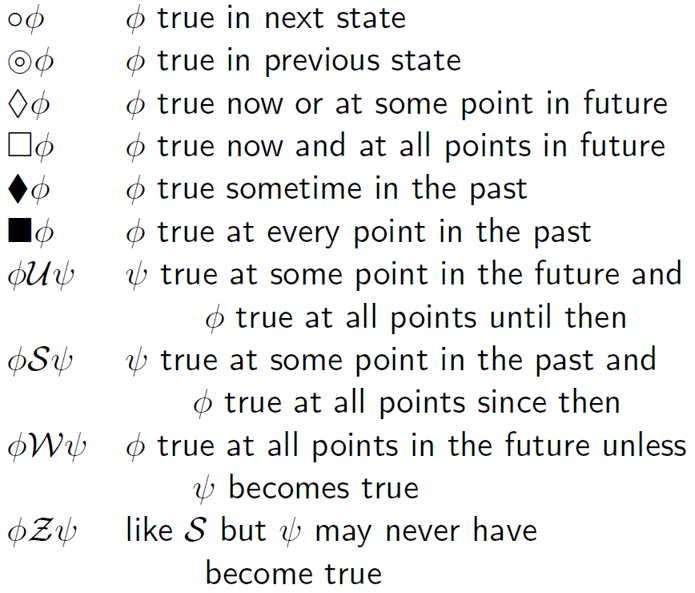
\includegraphics[width = \textwidth]{Images/Temporal_Logic_Symbols}
\end{figure}

\subsubsection{Concurrent MetateM}
\begin{itemize}
    \item Agents are specified as a set of temporal logic rules, permitted incoming arguments, and output types
    \item Each agent uses its history/incoming information to match against rules - on a match, it performs an action
    \item Concurrent agents can communicate with asynchronous messages
\end{itemize} 

At each state, the agent:
\begin{enumerate}
    \item Reads incoming messages to set state booleans
    \item Checks which rules fire in the current state
    \item Executes rules and fulfils any commitments from actions in previous states (commitments take priority)
\end{enumerate} 

This way, the agent separates immediate reactions with long term actions to achieve a goal. The reasoning is still difficult, as is translating the world to symbols. 

\subsection{Brookes: Subsumption Architecture}

\subsubsection{Concept}
This approach is heavily inspired by \emph{Behaviourism}, that a system can be described by how it reacts to its environment. 

It's primary principle is that real intelligence \textbf{must be situated in the real world}, and emerges from the interactions with the world. It can't be achieved by an abstract theorem solver.

Brookes put forward three theses:
\begin{enumerate}
    \item Intelligence can be generated without explicit representations
    \item Intelligence can be generated without abstract reasoning
    \item Intelligence is an emergent property of a complex system, rather than inherent/quantifiable
\end{enumerate}

\subsubsection{Composition}
The architecture is composed of sets of modules/rules/behaviours, each of which takes the form:
\begin{center}
    IF situation THEN action
\end{center}
These behaviours are organised into hierarchies to resolve ties. 

\subsubsection{Performance}
Though simple, it achieves near-optimal performance on multiple domains. However, it can't think ahead to future episodes, and doesn't have a history to reference. 

\subsection{Hybrid Architectures}
Some researchers have suggested an agent with two subsystems: one deliberative, one reactive. Usually the reactive takes priority.

To manage priorities, the system is split into layers:
\begin{description}
    \item[Horizontal Layering] Each layer is connected to the input and output, and each gives a separate suggestion - as if each were a separate agent
    \item[Vertical Layering] Layers are connected to each other (one connected to input, one to output), and take the results from the previous layer as input to make decision
\end{description}

Horizontal layering gives a wide variety but introduces a bottleneck as every layer must wait for the slowest. Vertical layering isn't tolerant to a single layer failing, but makes decisions across multiple layers than a single choice at the end. 

\section{Agent Based Modelling}
\textbf{Simulations} are an abstracted model of the real world. They can be used to test theories/effects of potential future changes, without actually implementing them. \\

They're widely used where data analytics fail.i.e in very complex systems, where behaviour is emergent, and where data isn't available. Simulations \emph{generate} data, rather than just analyse it.\\

\subsection{Models}
Any simulation uses a model, which is an abstraction of the real world made to be as simple as possible. Models are based on assumptions and theories, often to test the theories. \\

If a simulation/model explains a real-world phenomenon, then it is a \emph{candidate solution} - further proof is needed to call it a \emph{causal explanation}. The further proof is an ill-posed problem.\\

One test is to vary the initial parameters - fragile models are very sensitive, so will vary dramatically with a tiny change. 

\subsection{Bottom-Up Modelling}
Agent-based modelling is a \emph{bottom up} approach - the individual parts of the system are defined, and the behaviour of the system as a whole is emergent from the interactions of the parts. \\

These parts/agents can be heterogeneous - a single agent can then be individually changed, and the effects of that change are then transmitted to the system organically.

\subsection{Environment}
Agents are embedded into an environment, which define their behaviour.
\begin{description}
    \item [Spatial Models] Agents have co-ordinates on a grid, and can move about. Interactions are based on proximity.
    \item [Network Models] Links between agents are via edges, like a graph. Interactions are based on link proximity.
\end{description}
Environments can also contain non-autonomous entities, like the weather/ external factors.

\subsection{Scale and Feedback}
Since agents are non-deterministic, and behaviour emerges from interactions, every run of the system is unique. These can be from lots of simple agents, or a few behaviourally complex agents. e.g. Testing network effects at scale on simple agents vs. testing how a few agents react to a complex environment

The rich data obtained comes from feedback loops: the final state isn't a simple function of the initial state. These loops don't depend on the size/scale of the system, just its structure. 

\subsection{Cellular Automata}
A simpler system that influenced most ABM models. \begin{itemize}
    \item The environment is a grid of cells, and each cell has a state
    \item At each time step, the cell updates based on its neighbours' states
    \item Each cell is a non-moving, homogeneous agent with no memory in a fixed dynamic environment (i.e the neighbouring cells)
\end{itemize}
A famous example is Conway's Game of Life.

\subsection{Shelling's Segregation Model}
A precursor to ABM's, that focused on individuals in the system - their individual decisions had effects they neither intend nor were aware of. e.g people wanting to live amongst their community splits cities on racial lines

\subsection{Intervention}
An \emph{Intervention} is a change in the model that affects the agents behaviour. It can be explored by comparing the 'before' and 'after' applying the changes.

\subsubsection{Influence Maximisation}
By identifying which agents have most influence on the system (e.g the most connections in a network model), interventions can be targeted at them - this maximises the amount of change with minimal intervention. In the real world, these could be applying changes to social media influencers or targeted at certain ethnic/political groups.

\subsubsection{Influence/Spreading Functions}
Influence can be modelled in different ways, such as in peer pressure (an agent is influenced if a certain percentage of its connections are). The spread of disease can be modelled in such a fashion. 

\subsection{Creation}
Usually the agents are relatively simple (e.g. BDI, state machines, subsumption-based), and the behaviour emerges from their interactions. The agents only need to capture the relevant behaviour, so they don't need to be complex. \\

Data is required for realistic modelling:

\begin{itemize}
    \item Calibration - to set the initial agent/environment parameters
    \item Verification - use the data to set limits on the agent behaviour, etc.
    \item Validation - check the simulation is correct against real data (Face validation is checking against estimates)
\end{itemize}

\subsubsection{Pyschological Agents}
For social setting models, we simulate a particular aspect(s) of the psychology of the individuals. e.g wanting to do X\\

Adding psychological models such as stress and trust can increase the realism of the model - some models even have their agent learn and adapt as the model iterates (i.e. reinforcement learning)



\section{Coordination}

Agents are autonomous: so in a multi-agent environment, one agent can't \emph{force} another agent to taken an action. Instead, they have to communicate to try to influence other agents.

\subsection{Speech Acts}
The \emph{Speech Act Theory} (John Austin, 1962) states that communication is an action that aims to achieve an intention. The speech act can be split into three parts:
\begin{enumerate}
    \item Locutionary - making the communication. e.g. saying 'Open the Door'
    \item Illocutionary - conveying intentions (highly context dependent)
    \item Perlocution - the effect of the communication. e.g. the door has been opened
\end{enumerate}
Agents make a locutionary act, hope that the illocutionary act has been transmitted (i.e the speaker understood the meaning), and expect the listener to effect the perlocution. 

\subsubsection{Classes of Speech Acts}
According to John Searle (1969), there are five classes:
\begin{description}
    \item [Representative] The speaker says a statement is True/False. e.g. it is raining, it is not 5pm
    \item [Directive] The agent asks the hearer to do something
    \item [Commissive] The agent commits to doing something. e.g. I will submit it by 6pm
    \item [Expressive] The speaker expresses a mental state. e.g. 'Thank you', 'I am sad'
    \item [Declaration] The speaker says something, which causes an effect. i.e the speech is an action. e.g. 'We are now at war with Mars'
\end{description}

\subsubsection{Parts of a Speech Act}
Speech acts have two components:
\begin{description}
    \item [Performative Verb] The illocutionary part. e.g. request, inform, commit
    \item [Propositional Content] The raw content
\end{description}
e.g.
\begin{table}[H]
\centering
\resizebox{\textwidth}{!}{%
\begin{tabular}{|l|l|l|l|}
\hline
                            & Verb: Request         & Verb: Inform       & Verb: Inquire       \\ \hline
Content: The door is closed & Please close the door & The door is Closed & Is the door closed? \\ \hline
\end{tabular}%
}
\end{table}

\subsection{Agent Communication Languages}
Provide a standardised way for heterogeneous agents to communicate. 

e.g. the KQML is an agent communication language that consists of a Knowledge Interchange Format (to denote info/relationships) and a Knowledge Query Manipulation Language (to define performatives). Agents apply the latter to teh former (as in speech acts) to communicate. 

\subsubsection{Communication as Actions}
Communication is treated as a separate action in a plan. e.g Request(X,Y,Z):
\begin{description}
    \item [Preconditions] X believes Y can do Z, X wants Y to do Z
    \item [Effect] X believes Y wants to do Z
\end{description}


\subsubsection{Communication as Mental States}
Communications are based around the beliefs of an agent. i.e. if an agent believes a fact to be true

The effect isn't caused as soon as the communication occurs, leading to a potential difference between what the agent believes and what is true.

\subsubsection{Communication as Social Commitments}
Communications are transmitted as commitments from one agent to another. e.g. If I tells J that $\neg A$, then it can't tell K that $A$ unless it also tells J

These commitments can be publicly verified. 

\subsubsection{Effectiveness}
\begin{itemize}
    \item Most of these approaches assume the agents share the same semantics/thought processes as well as the semantics - not always feasible
    \item Limited to the set of 5 performatives - we can expand this list, but where do we stop?
    \item As a positive, these performatives act as shortcuts to more complicated concepts
\end{itemize}


\subsection{Co-operation}
Agents are autonomous. i.e they make decisions at runtime. Therefore, any co-operation between them must be dynamic, rather than hard-wired

\subsubsection{Measuring Co-operation}
Bond and Gasser [1992] proposed the following criteria to evaluate cooperation:
\begin{description}
    \item [Coherence] How well the system achieves the goal. e.g. outcome measure, time taken
    \item [Co-ordination] How well the agents work together. e.g. not getting in each other's way, sychronizing routines so they're not waiting for each other
\end{description}

\subsubsection{Co-operative Distributed Problem Solving}
A type of domain where agents are autonomous and can solve different problems independently, but must work together to complete the problem as a whole.
\begin{itemize}
    \item No agent has enough knowledge/skills by itself
    \item The problem is modular (can be split into reasonable blocks)
    \item More time spent on computation than communication (if the other way, better to make one 'super' agent)
\end{itemize}

Solving a CDPS problem has 4 main steps:
\begin{enumerate}
    \item Decompose the problem \\ \quad \quad - Which agent decomposes, and how granular is the decomposition?
    \item Allocate the subproblems \\ \quad \quad - Who decides the allocations? What if an agent refuses its allocation?
    \item Solve the subproblems \\ \quad \quad - Some subproblems might need scheduling/further co-operation
    \item Combine the subproblem solutions as required
\end{enumerate}

\subsubsection{Contract Net Protocol}
A protocol to allocate subproblems, where the agents bid for the problems they want. The process is:
\begin{enumerate}
    \item An agent recognises a problem needs co-operation/delegation of parts
    \item Agent broadcasts the task: - description, constraints (e.g. deadline) and meta-information (e.g. bid submission deadline)
    \item Other agents consider, and maybe return a bid
    \item First agent decides who gets the task, and informs all the bidders
    \item The winning agent (contractor) performs the given task
\end{enumerate}

In an ACL, this would be: agent calls for proposal, other agents propose, agent accepts/refuses to all other agents, contract informs of failure/success of task.\\

The collection of agents is the contract net - the only hierarchy is the delegation of tasks, otherwise all agents are equal. e.g A delegates X to B, B splits X into X$_1$ and X$_2$, delegates X$_1$ to A and X$_2$ to C \\

The protocol works well for distributed data, heterogeneous agents (with different skills), and tasks large enough to split and delegate. 

\subsubsection{Co-ordination, Multi-agent Planning and Joint Intentions}
Co-ordination is managing dependencies between agents activities.
\begin{description}
    \item [Positive] Agents ask for help with actions, don't plan the same actions, contribute to others' actions
    \item[Negative] Agents try to use resources at the same time, plan actions that require other agents even if they're busy
\end{description}

One way to manage co-ordination is through various types of \emph{Multi-Agent Planning}: 
\begin{description}
    \item[Centralised Planning] A central agent makes plans for all agents
    \item[Merging] Each agent makes a plan, and a central agent merges them to produce a global plan
    \item[Partial Global Planning] Each agent receives the global plan, makes its own plan accordingly and adjusts the global to include the new information, then passes the global plan along - no centralised system
\end{description}
Multi-agent planning requires agents to share private info and reduces autonomy. Combining plans is also non-trivial.\\ 

\emph{Joint Intentions} is a teamwork-based approach. Agents have shared goals, and a responsibility towards other agents. Every agent works towards a goal G with a motivation M - if G is no longer possible or M doesn't hold, the agent tries to inform the other agents. If G is achieved, it instead informs the other agents that the goal is over. 

\subsection{Expectations and Norms}
To co-ordinate, agents need to have expectations on how other agents will act. These can be obtained via:
\begin{enumerate}
    \item Communications and joint intentions
    \item Knowledge of the system: what is normal/required, past experiences (trust) and reputation of other agents
\end{enumerate}

\subsubsection{Normative Agent Systems}
A \emph{norm} is an expected pattern of behaviour - it isn't guaranteed though. They can be \emph{Conventions}(e.g. take a gift when visiting people) or \emph{Prescripted} (e.g. follow the laws). \\

A prescriptive norm can be formally represented with: who it affects, is it an obligation/permission/prohibition, when it applies, what it is, and what the punishment for breaking it. e.g. 
\begin{center}
    $<$All Drivers, Obligation, At a red light, Stop, 3 points on licence$>$ 
\end{center}
\subsubsection{Reasoning with Norms}
Norms affect agent behaviour: violating one has a punishment and causes a loss of reputation, so agents will add achievement/maintenance tasks to not break norms. For MAS, agents can expect other agents to generally follow norms - but this isn't guaranteed. \\

Agents might break norms if: they didn't know/understand, the punishment is too low, another norm/goal is more important, or if the norms aren't being enforced. \\

\subsubsection{Conventions as Emergent Behaviour}
Conventions can occur from agents copying other agents - these might not be globally followed, with different subsets of agents following different norms. e.g driving on the right/left\\

By applying influence maximisation, desired norms can be spread across agents by targeting influencers.


\subsection{Trust/Reputation}
Agents running a bid will pick the agent it believes will do the best job (maximising expected utility). This belief can either come from previous dealings with the agent in question (\textbf{Trust}), or by the trust from other agents (\textbf{Reputation}). \\

Reputation requires trust in the other agents' ratings: the ratings could be on a different scale, or two agents could collude to boost their reputation with other agents.e.g fake amazon reviews. 

If the agent only uses trust, it will continuously pick the same agent as it never generates trust scores for unknown agents. A degree of exploration can be built into the agent, so it tries new agents and generates new trusts.

\subsubsection{FIRE Model}
One example of trust/reputation is the FIRE model - it uses a weighted sum of:
\begin{itemize}
    \item Direct experience
    \item Other trusted agent references
    \item Norm expectations
    \item References provided by the agent
\end{itemize}
The weights are based on the source and recency of the information. 


\section{Negotiation}
Self-interested agents need to agree on how to perform/allocate tasks/resources - they do this by negotiating.

An \emph{Agreement Protocol/Mechanism} defines the structure of the negotiation/argument:
\begin{enumerate}
    \item What moves each agent can make
    \item What are the permitted responses/sequence of moves. e.g. can an agent make an offer in response to an offer?
    \item How the outcome is determined
\end{enumerate}
Each agents has a \emph{Strategy} to decide what move it makes in a given state. 

\subsection{Game Theory}
A way to analyse negotiations/scenarios where each agent tries to maximise its own utility. 
\begin{description}
    \item[Strategy] The action the agent chooses to take
    \item[Outcome] The result of each agent/player executing their action
    \item[Dominant Strategy] No matter what the other player(s) do, this is the best strategy for an agent
    \item[Nash Equilibrium] An outcome where no agent benefits from changing, assuming no other agent changes
    \item[Pareto Optimal] An outcome where changing to any other outcome to benefit one player would harm another player(s)
    \item[Max. Social Welfare] The outcome with the max. utility sum across all agents
\end{description}
e.g.
\begin{table}[H]
\tiny
\centering
\resizebox{\textwidth}{!}{%
\begin{tabular}{|c|c|l|l|}
\hline
 Agents &  & \multicolumn{2}{c|}{Agent 2} \\ \hline
 & Actions & \multicolumn{1}{c|}{A} & \multicolumn{1}{c|}{B} \\ \hline
\multirow{2}{*}{\begin{tabular}[c]{@{}c@{}}Agent \\ \\ 1\end{tabular}} & A & \begin{tabular}[c]{@{}l@{}}\quad \quad2\\ 2\end{tabular} & \begin{tabular}[c]{@{}l@{}}\quad \quad4\\ 0\end{tabular} \\ \cline{2-4} 
 & B & \begin{tabular}[c]{@{}l@{}}\quad \quad0\\ 4\end{tabular} & \begin{tabular}[c]{@{}l@{}}\quad \quad0\\ 0\end{tabular} \\ \hline
\end{tabular}%
}
\end{table}
In the above example of a game with two agents and two actions each: BB is the Nash Equilibrium; AA, AB and BA are Pareto Optimal; AA, AB and BA maximise Social Welfare. 

\subsection{Properties of Agreement Mechanisms}
An agreement mechanism can be any of the following:
\begin{enumerate}
    \item Individual Rational - No agent is worse off for participating
    \item Symmetric - Same rules for everyone
    \item Fair - Every agent has an equal chance of affecting the outcome
    \item Pareto Optimal - A PO outcome is guaranteed
    \item Maximises social utility - An outcome that maximises social utility is guaranteed
    \item Stable - A Nash Equilibrium Exists
    \item Simple - easy to find the best strategy
    \item Guaranteed to terminate - no way the participants interact indefinitely 
\end{enumerate}

\subsection{Negotiation Definitions}
Negotiations usually take place over a series of rounds, and each agent makes one proposal per round. The \emph{Negotiation Set} is the set of possible proposals that an agent can make.

Negotiations can be \emph{single-issue} (e.g. the price of X) or \emph{multi-issue} (e.g a contract with multiple clauses). In the single it's obvious where concessions are made, but in the multi it's not obvious how the various issues relate. Multi-issue negotations also can't be simply iterated over, as there are too many possibilities. 

Negotiations can be one-to-one, many-to-one (e.g an auction) or many-to-many.

\subsection{Alternating Offers Protocol}
A one-to-one protocol to split a given amount - in each round, one agent proposes a deal and the other either accepts (and the negotiation terminates) or rejects and continues to a new round with the roles reversed.

The game is not guaranteed to terminate: if the agents can't reach a deal, this is known as the \emph{Conflict Deal} - which is the worst possible outcome for both agents. 

\subsubsection{Ultimatum Game}
Like the AoP, but only a single round. Guaranteed to terminate, but unfair to agent 2 as only agent 1 can affect the outcome (both want to avoid a conflict deal)

\subsubsection{Strategies}
Given that all agents want to avoid a conflict deal, the agent going last (with a fixed number of rounds) can offer any deal, and the other agent must accept. For an indefinite number of rounds, the first agent will get any deal they want - as they always go first, they can propose the same deal every time and reject whatever the second agent proposes. \\

Agents are generally impatient - the sooner they get something, the more value it has. This can be represented as the value of X to agent i at round K being $\delta^k_i \cdot X$ - the higher $\delta_i$, the more patient agent i is.\\
Knowing the patience of the other agent allows you to make an offer they must accept - the longer the game goes on the less the item is worth to them. For an indefinite number of rounds, the deal agent 1 should make (Assuming the split is (agent 1, agent 2)) is:
\[
    \left( \frac{1-\delta_1}{1-\delta_1\delta_2},\frac{\delta_2(1-\delta_1)}{1-\delta_1\delta_2} \right)
\]

\subsection{Task Oriented Domains}
Agents have to achieve a set of tasks: they can negotiate to swap tasks to be more efficient. The domain is represented as: \textbf{$<T,Ag,c>$} = $<$set of tasks, set of agents, cost of each subset of tasks$>$. 
\begin{itemize}
    \item Encounter - Initial allocation of tasks (a set $<T_1,T_2,...,T_i>$ where $T_i$ is the allocation for agent i)
    \item Deal - The final allocation of tasks(a set $<D_1,D_2,...,D_i>$ where $D_i$ is the allocation for agent i)
    \item Cost of deal for agent i - $c(D_i)$
    \item Utility of deal for agent i - $c(T_i) - c(D_i)$
    \item Conflict Deal - the initial deal
    \item Individual Rational Deal - a deal where no agent prefers the conflict deal
\end{itemize}
The negotiation set is all deals that are individual rational + pareto optimal (i.e utility $>= 0$ for all agents)

\subsubsection{Deception}
Agents can lie about the number of tasks they have to get a better deal. 
\begin{enumerate}
    \item Hidden Task - An agent can hide a task from its encounter. This lowers the encounter cost, so reduces the individual rational strategies to give it a better deal
    \item Phantom Task - An agent can pretend to have been allocated a new task. This task can make another task (which the agent wants) look worse, so no other agent will bid for it. 
\end{enumerate}

\subsection{Monotonic Concession Protocol}
One-to-one protocol: agents simultaneously propose deals in each round. If neither agent agrees to its opponent's deal, the round continues - in the next round, each agent's proposed deal \emph{cannot be less preferable to it's opponent}. i.e it must propose a deal that is equal/better for the other agent. If neither agent concedes on their deal, the conflict deal is chosen.

\subsubsection{Zeuthen Strategy}
\begin{enumerate}
    \item The first deal an agent proposes is its most preferred
    \item The agent least willing to risk conflict should conceded
    \item An agent should only concede enough to change the balance of risk
\end{enumerate}
This strategy maintains a Nash Equilibrium, so agents can announce this strategy without losing anything. \\

The closer an agent's deal is to the conflict deal, the more willing to risk (less to lose). 
\begin{align*}
    \text{A's willingness to risk} &= \frac{utility(Deal_a) - utility(Deal_b)}{utility(deal_a)} \nonumber \\
    &= \frac{\text{Utility lost by conceding}}{\text{Utility lost by conflict}} \nonumber
\end{align*}
If $utility(deal_a)$ = 0 (i.e. the conflict deal), then the risk = 1.
\section{Voting}
\emph{Social Choice Theory} is the study of how group decisions are made. Agents are self-interested and want to influence the outcome in their favour, so they use voting protocols to account for a range of preferences.

\subsection{Domain}
There are a set of N \emph{voters}, each of which have preferences to a set of \emph{outcomes/candidates}. We assume that each voter has a complete set of preferences($A>B or B>A \forall (A,B)$, and that these preferences are transitive ($A>B,B>C\rightarrow A>C$) - so we can represent them as a ranked list.

\subsection{Preference Aggregation}
Given a collection of preference orders, combine them into an ordering that reflects the orders as closely as possible. There are two main types of algorithm:
\begin{description}
    \item[Social Welfare Function] combine the data into a new complete ordering
    \item[Social Choice Function] combine the data to select a single most preferred outcome
\end{description}

\subsection{Plurality Voting}
A simple social choice function: each outcome gets one point if it's \textbf{first} in a voter's preference ranking, and the outcome with the most points is selected.\\
This ignores the rest of the preference/lower ranks. e.g. voters are split between A and B for first, but everyone has C in second. It also allows for strategic voting: if an agent knows the rankings of other agents, it can submit a false ranking to change the outcome.

\subsection{Condorcet Winner}
A social choice function: every pair of outcomes has a contest, and the outcome that beats \emph{every} other outcome is chosen. The contest is simply the number of voters that prefer one outcome to the other. i.e. for (a,b), a gets +1 point for each voter with $a>b$ and -1 for each voter otherwise

\subsubsection{Condorcet Principle and Paradox}
Any system that follows the \emph{Condorcet Principle} will always choose the condorcet winner. However, there might not be a candidate that wins in every case - this is the \emph{Condorcet Paradox}.

\subsection{Linear Sequential Majority}
A social choice function: outcomes take place in pairwise rounds, and the winner moves onto the next round. e.g. (4,3) $\rightarrow$ winner faces 1 $\rightarrow$ winner faces 2 \\
The order of the contests is called the \emph{agenda} - it determines which outcomes face each other, and is open to manipulation as some outcomes might not be the strongest, but if they're at the end of the agenda can still win. The contests can be represented as a \emph{majority graph}, with an edge $a\rightarrow b$ implying a beats b in a simple majority. 

\subsection{Instant Run-Off}
A social choice function: in each round, the candidate with the least number of first choice votes is removed from all voters' lists, and this continues until only one outcome remains. If a voter's first choice is removed, then its second choice becomes its first and so on. \\
This method doesn't account for deeper preferences in candidates that are removed early. e.g. nobody had B first, but everyone had them second.

\subsection{Copeland Rule}
A social choice function: similar to condorcet, except the outcome with \emph{the most wins} is chosen. i.e. there doesn't need to be an outcome that beats every other outcome. A win gives 1 point, a loss -1 points, and a draw 0.

\subsection{Borda Count}
A social choice function: similar to plurality but the full ranking is used, with each position being weighted. The outcome with the most points wins. The weighting for m candidates is: (m-1) points for each first place vote, (m-2) for each second place \dots 0 for last place votes.

\subsubsection{Spoiler Effect}
Candidates who don't win the election under the borda count can still shift the results of the election.e.g.
\begin{center}
    3 votes for $a>b$, 2 votes for $b>a$ - a wins \\
    3 votes for $a>b>c$, 2 votes for $b>c>a$ - b wins 
\end{center}
This happens because B now receives more votes as it's not in last place, while A still is. 

\subsubsection{Positional Scoring}
Rather than strictly (m-1), (m-2), the scores ($S_1,S_2,S_3,\dots,S_m$) can be any values as long as the following two rules are maintained:
\begin{enumerate}
    \item $S_1 \geq S_2 \geq S_3 \geq \dots \geq 0$. (Non-negative decreasing scores)
    \item $S_1 \ge S_m$. (The scores must decrease at some point) 
\end{enumerate}
e.g. $S_m = 0, S_{m-1} = 1, S_{m-2} = 3, S_{m-3} = 6, S_1 = m (m+1)/2$
Positional scoring as a whole violates the condorcet principle (i.e. it's not always guaranteed to provide the condorcet winner)

\subsection{Voting Rule Properties}
\begin{description}
    \item[Anonymous] All votes are counted equally  - no voter is more influential than any other
    \item[Resolute] A unique winner (no ties)
    \item[Surjective] Every candidate has a chance to win
    \item[Dictatorship] there is a voter whose first choice is always the winner
    \item[Strategy-Proof] there isn't an ordering for a voter that gives it a better outcome than its true preferences (no reason for a voter to lie)
    \item[Weakly Pareto] It won't select an outcome A it there is an outcome B such that $B>A$ for all voters
\end{description}

\subsubsection{Gibbard-Satterthwaite Theorem}
Any resolute, surjective and strategy-proof rule for 3 or more candidates will be a dictatorship.\\
Selecting a strategy can be very difficult, so this doesn't mean that all rules are inherently useless.

\subsubsection{Independence of Irrelevant Alternatives}
The outcome of a preference between A and B should only depend on the preferences between A and B. e.g. if $A>B$, then adding C shouldn't change that. As seen previously, the Borda Count does not hold IIA

\subsubsection{Arrow's Impossibility Theorem}
Any rule that is surjective and is independent of irrelevant alternatives will be a dictatorship.

\subsubsection{Universal Domain Assumption}
Both of the above theorems assume that every voter has a complete preference ordering - if we drop this assumption, then the theorems no longer hold.

\subsection{Median Voter Rule}

\subsubsection{Single-Peaked Preference}
There is an ordering over the outcomes, and outcomes closer to your first choice are more preferred than those further away. e.g. let the outcomes be 21,17,11 and 4 - if a voter chooses 17, they'll prefer 21 to 11. 

\subsubsection{Voting Rule}
A social choice function: each voter chooses a single candidate, the votes are ordered, then the median candidate is chosen. e.g. 
\begin{center}
    21 gets 10 votes, 17 gets 20 votes, 11 gets 40 votes, 4 gets 30 votes. \\
    There are 100 votes in total, so the median is 50 - this is 11, so 11 is the winner
\end{center}
If there are an odd number of voters, this provides a condorcet winner. The rule is strategy proof (a voter can't shift the median towards their true outcome by voting against it), and is weakly pareto.
\section{Auctions}
\emph{Auctions} are a mechanism to allocate \textbf{limited} resources that are desired by more than one agent. The resources are allocated based on how much each agent values the resource.

\subsection{Structure of an Auction}
\subsubsection{Types of Agents}
\begin{description}
    \item[Auctioneer] an agent that allocates the resources - wants to maximise the selling price
    \item[Bidder] an agent that wants to minimise the price they pay for the resources - they do this by using a \emph{strategy} to place bids
\end{description}

\subsubsection{Valuation of Goods}
\begin{description}
    \item[Public/Common] The good has the same value to all agents - but not all agents have perfect information on this value
    \item[Private] Each agent has their own value on the good. e.g. sentiment
    \item[Correlated] Private + based on other people's valuations. e.g. buy a good to sell it later, so you need to know how much others want it
\end{description}

\subsubsection{Visibility of Bids}
\begin{description}
    \item[Open Cry] Bids are common knowledge to all bidders
    \item[Sealed Bid] Bids are private
\end{description}

\subsubsection{Bidding Mechanism}
\begin{description}
    \item[Ascending/Descending] Start at price X, subsequent bids increase/decrease the price
    \item[One-Shot] All agents submit a single bid
\end{description}

\subsubsection{Winner Price Determination}
\begin{description}
    \item[First Price] Agent with the highest bid pays the highest bid
    \item[Second Price] Agent with the highest bid pays the second highest bid value
\end{description}

\subsection{English Auctions}
First price, open cry, ascending. The bidding stops after a set time deadline or a fixed time period in which no bids have been made. 

\subsubsection{Bidder Strategy}
Agents will never bid more than their expected value of the good. Instead, they bid $\Delta V$ (the smallest permitted amount) above the current highest bid until they reach their expected value.

\subsubsection{Expected Price}
The auctioneer will receive the second highest bid + $\Delta V$, as opposed to the winner's true valuation. It therefore loses out that much. The less competition, the higher the loss of revenue for the auctioneer.\\
Auctioneers (or agents they collude with) can place \emph{shill bids}, which are false bids intended to drive up the value of the second highest bids. Auctioneers will also have a \emph{reserve value}, which is the minimum value they will sell for. 

\subsection{Dutch Auction}
First price, open cry, descending. The auctioneer controls the speed of the descent, and the first bidder to accept the current price wins. 
\subsection{Bidder Strategy}
Agent will never bid more than the expected value. Below this value, the agent needs to balance two risks: decreasing the price vs. losing the item to another agent. This is made harder as the agent doesn't know the valuations of the other agents. 

\subsubsection{Risk Attitudes}
\begin{description}
    \item[Risk Averse] An agent that's less likely to take risks
    \item[Risk Seeking] An agent that's more likely to take risks
    \item[Risk Neutral] An agent that bases their choice solely on probabilities. e.g. 
\end{description}

\subsubsection{Expected Price}
If the bidders are risk averse, they will accept as soon as it hits their true value, so the auctioneer will get the maximum valuation across all agents. If they're risk-seeking, then an English Auction provides better results.

\subsection{First Price Sealed Bid}
A one-shot auction mechanism, where every agent submits one private bid. It's similar to a dutch auction - agents won't pay more than their true valuation, and below that depends on their risk attitude.\\

All of the mechanisms so far have bidders taking into account the other agent's valuations, rather than giving their true valuations.

\subsection{Vickrey Auction}
Second price, sealed bid, one shot. As agents only pay the second price, it might be possible to bid more than their true valuation

\subsubsection{Bidder Strategy}
\begin{itemize}
    \item If they bid higher than their true value, the second bid could also be higher - this would end in a loss
    \item If they bid lower than their true value, they have less chance of winning and they still get the second highest valuation
\end{itemize}
Therefore, it makes sense for the bidders to bid their true values

\subsubsection{Expected Price}
Auctioneers will get the second highest true valuation - this is slightly less than an english auction.\\

An \emph{anti-social bid} is a bid placed to intentionally raise the second highest bid, so the winner pays more. This is risky for a bidder this value will be higher than its true valuation, so it might accidentally win and get a loss. However, an auctioneer can place a shill anti-social bid at no risk once it knows the highest bid.

\subsection{Winner's Curse}
For any auction, the winner always faces the concern that they paid too much/over-valued the good, as no other agent was willing to pay that much. This is especially the case if the good has a public value. For a Vickrey auction this is reduced, as the second highest agent would have also needed to imperfectly value the good.

\subsection{Bidder Collusion}
Multiple/all of the bidders could collude to buy the good at a low price, then sell it elsewhere for a higher price and split the profits between them.\\
This is dangerous if the agents cant trust each other, as one could betray and buy it for a slightly higher price then keep it. Hiding agent bids and keeping who wins a secret further dicourages collusion.

\subsection{Combinatorial Auctions}
Auctions in which multiple goods are auctioned at the same time. For the set of goods Z, each agent i$\in$Ag has a preference/valuation function over subsets of goods ($v_i: 2^Z\rightarrow{R}$(real numbers)). The outcome of the auction is the set of allocations of each item (${<z^*_1,z^*_2,\dots>}$) - an item can't be allocated to more than one agent. 

\subsubsection{Properties of Valuation functions}
\begin{description}
    \item[Free disposal] the agent isn't worse off getting more items ($z_1\subseteq z_2\rightarrow v_i(z_1) \leq v_i(z_2)$ )
    \item[Normalised] $v_i(\emptyset )=0$
    \item[Substitutable] Some goods can replace others, so we don't want to repeat items. e.g. buying a console+game and buying just the game \\ \qquad \qquad $z_1 \cap z_2 \neq \emptyset ,\quad v_i(z_1) + v_i(z_2) > v_i(z_1 \cup z_2)$
    \item[Complementarity] Some goods increase in value when together. e.g. 2 halves of a set of collectable items
    \\ \qquad \qquad $z_1 \cap z_2 \neq \emptyset ,\quad v_i(z_1) + v_i(z_2) < v_i(z_1 \cup z_2)$
\end{description}
The \emph{exposure problem} is when an agent bids high for all of the items in a complementary set, but fails to obtain one or more - they've now overpaid for the other items. 

\subsubsection{Maximising Social Welfare}
The auctioneer wants to maximise social welfare (give each bidder its highest valuation), but doesn't have access to the valuation functions of each agent. Even if each agent declares its entire value function, this isn't sufficient as:
\begin{enumerate}
    \item Agents can lie on their value functions
    \item The table would be of size numOfAgents x numOfBundles. For 1000 items, there are more possible combinations than atoms in the universe
    \item Np-hard problem, even assuming a small number of items/agents
\end{enumerate}

\subsubsection{Bidding Language}
Agents can submit \emph{atomic bids} - a pair (z, p) of a bundle and the price the agent is willing to pay for it. This defines a valuation function $v_i$ where $v_i(z') = p$ if $z'\supseteq z$, and $v_i(z') = 0$ otherwise.\\
These can be connected with an XOR to form \emph{composite bids} - agents will pay for one of the atomic bids to be satisfied. If multiple bids are, then the agent pays the highest price. These composite bids can be used to represent the entire set of possible bundles, and only require an exponential amount of atomic bids if the agent has a different valuation for every combination of goods. e.g. if the agent only wants a good g, then it can represent every bundle containing that good with a single atomic bid

\subsubsection{Winner Determination Problem}
This is a combinatorial optimisation problem, which is NP-Hard. To make the problem easier we can
\begin{enumerate}
    \item Restrict the number/types of bids - constraints
    \item Use different techniques for specific cases - heuristics
    \item Accept approximate solutions
\end{enumerate}
One set of constraints is to limit the size of bids, and say that the bids must be on a continuous set of good. e.g. continuous frequency spectrum. If there is no natural ordering, we can impose an artificial one.\\
An example of a heuristic is a greedy algorithm on bid prices - at each iteration, allocate the bundle with the highest bid price among all agents

\subsubsection{Vickery-Clarke-Groves Mechanism}
\begin{enumerate}
    \item Each agent declares their valuation function
    \item The auctioneer allocates to maximise social welfare $\rightarrow{<z^*_1,z^*_2,\dots>}$
    \item For each agent i, the price is $p_i$ where:
    \begin{enumerate}
        \item Determine the max. social welfare allocation if i wasn't present  $\rightarrow{<z'_1,z'_2,\dots>}$
        \item \begin{align*}
                p_i &= \sum_{k\in (Ag\neq i)}v_k(z'_k) - \sum_{k\in (Ag\neq i)}v_k(z^*_k) \\
                    &= \text{social welfare lost since the agent is present}
            \end{align*} 
    \end{enumerate}
\end{enumerate}

\section{Argumentation}
An \emph{argument} is a reason to believe/do/want something.
\begin{itemize}
    \item Can be exchanged between agents to resolve differences and structure interactions
    \item Agents can use them to structure their internal reasoning
    \item There can be multiple arguments for/against the same thing
\end{itemize}

An argument is structured as a set of \emph{premises} to support a \emph{claim}. i.e X because Y,F and M

\subsection{Definition}
\emph{Argumentation} is the process of constructing/exchanging arguments to interact with other agents.
\begin{enumerate}
    \item Abstract Argumentation - given a set of arguments that contradict each other, find a consistent set of knowledge
    \item Argument-based Dialogue - give a standard structure for interaction in negotiation, persuasion, etc.
\end{enumerate}

\subsubsection{Terms}
\begin{description}
    \item[Database] a set of formulae/knowledge, might not be internally consistent
    \item[Argument] (premises,claim) - the premises are present in the database, and the claim follows from the premises (using classical logic). The premises are the minimal required set to prove the claim.
    \item[Attack] when two arguments conflict with each other
    \begin{description}
        \item[Rebut] $(p_1,a_1)$ and $(p_2,a_2)$, where $a_1 = \neg a_2$ 
        \item[Undercut] $(p_1,a_1)$ and $(p_2,a_2)$, where $a_1 = \neg p$ for some $p\in p_2$ 
    \end{description}
\end{description}

\subsection{Abstract Argumentation}
The internal structure of the arguments are ignored, and the focus is on which arguments attack each other - this is represented as an attack graph (A,R) (= (arguments, attacks)).\\

An argument is \emph{In} if all attacking arguments are \emph{Out}, and \emph{Out} if any argument that attacks it is \emph{In}. Arguments can also be unlabelled. e.g. if $A\rightarrow{B}$ and $B\rightarrow{A}$, without making an assumption/external arguments then neither argument can be labelled.\\

An argument that isn't attacked by anything is \emph{In} by default. 

\subsubsection{Semantics}
    \begin{enumerate}
        \item Grounded Semantics - strictly follow the rules to minimise node labelling
        \item Preferred Semantics - Use assumptions to maximise node labelling
        \begin{enumerate}
            \item Preferred Credulous - an argument is marked In under any of the preferred labellings
            \item Preferred Sceptical - an argument is marked In under all of the preferred labellings
        \end{enumerate}
    \end{enumerate}

Preferred semantics are preferred as they provide us with more information to use.

\subsubsection{Subjective Defeat Relations}
For $A\rightarrow{B}$ and $B\rightarrow{A}$, A only \emph{defeats} B if A is subjectively preferred to B - introduces preferences for certain arguments.\\
These preferences can be explicitly shown in the graph, and can attack attack relations between arguments (e.g. in the above example, a preference for A would attack $B\rightarrow{A}$). Preferences can also attack each other or, or attacks on preferences, or \dots 

\subsubsection{Defeasible Knowledge}
Knowledge can be revised, attacked, or rendered void. If counter-evidence is provided, something assumed to be true can be changed to false. The above only applies to facts - opinions can't be objectively defeated. 

\subsection{Non-Monotonic Reasoning}
Agents can change their conclusions as they learn about the world - they can shrink or grow their set of conclusions (can only grow in monotonic). \\

Classical logic doesn't work well to represent this, but argumentation naturally allows for new knowledge to attack previous knowledge. It also provides simple/intuitive ways for humans to add in knowledge, and clearly shows why agents have taken certain decisions.

\subsection{Argument Dialogues}
Different agents can engage in dialogues with each other, to share their reasons and try to change the other agents' views. Arguments dialogues can be split into: initial situation/cause, , goal of the argument, and personal aims of the agents.

\subsubsection{Dialogue types}
\begin{table}[H]
\centering
\resizebox{\textwidth}{!}{
\begin{tabular}{|l|l|l|l|}
\hline
Type & Initial Situation & Main Goal & Personal Aims \\ \hline
Persuasion & Conflicting points of view & Resolution of views & Change the other agent's views to their own \\ \hline
Inquiry & Ignorance of multiple agents & Growth of knowledge & Find/destroy a proof/incorrect belief \\ \hline
Deliberation & Need for action & Reach a decision & Influence the outcome towards the 'best' \\ \hline
Neogtiation & \begin{tabular}[c]{@{}l@{}}Conflict of interests, \\ but co-operation required\end{tabular} & Make a deal & Get the best deal \\ \hline
Info-seeking & Ignorance of a single agent & \begin{tabular}[c]{@{}l@{}}Spread knowledge \\ (general/about other agents)\end{tabular} & Gain/Hide/Show personal knowledge \\ \hline
\end{tabular}
}
\end{table}

\subsubsection{Dialogue System}
The system is defined by:
\begin{enumerate}
    \item The moves each agent can make. e.g. assert, accept, challenge, question
    \item Protocol - rules on what moves can/can't be made. e.g. you can't attack an argument you made previously, you must accept arguments you can't attack
    \item Strategy for each agent - the 'best' strategy is still a research question
    \item When the argument terminates and determining the outcome. e.g. last argument wins
\end{enumerate}

\end{document}
